\documentclass[../main.tex]{subfiles}
\begin{document}
\chapter{Abstract Data Structures}
\label{chapter_abstract_data_structure}
(put a figure here)


\section{Introduction}
\label{chapter_abstract_data_structure_introduction}
Leaving alone statements that ``data structures are building blocks of algorithms'', they are just mimicking how things and events are organized in real-world in the digital sphere. Imagine that a data structure is an old-schooled file manager that has some basic operations: searching, modifying, inserting, deleting, and potentially sorting. In this chapter, we are simply learning how a file manager use to `lay out' his or her files (structures) and each `lay out's corresponding operations to support his or her work. 

We say the data structures introduced in this chapter are \textit{abstract} or idiomatic, because they are conventionally defined structures. Understanding these abstract data structures are like the terminologies in computer science. We further provide each abstract data structure's corresponding Python data structure in Part.~\ref{part_program_and_python}.

There are generally three broad ways to organize data: Linear, tree-like, and graph-like, which we introduce in the following three sections.

\paragraph{Items} We use the notion of \textbf{items} throughout this book as a generic name for unspecified data type.

\paragraph{Records}
%%%%%%%%%%%%%%%%%%%%%%%%%%%%%Linear%%%%%%%%%%%%%%%%%%%%%%%%%%%%
\section{Linear Data Structures}
\label{chapter_abstract_data_structure_linear_data_Strcuture}
\subsection{Array}
\begin{figure}[h!]
    \centering
    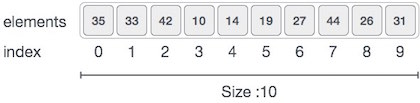
\includegraphics[width=0.7\columnwidth]{fig/array_representation.png}
    \caption{Array Representation}
    \label{fig:array_representation}
\end{figure}
\paragraph{Static Array} An array or static array is container that holds a \textbf{fixed size} of sequence of items stored at \textbf{contiguous memory locations} and each item is identified by \textit{array index} or \textit{key}. The Array representation is shown in Fig.~\ref{fig:array_representation}. Since using contiguous memory locations, once we know the physical position of the first element, an offset related to data types can be used to access any item in the array with $O(1)$, which can be characterized as \textbf{random access}. Because of these items are physically stored contiguous one after the other, it makes array the most efficient data structure to store and access the items. Specifically, array is designed and used for fast random access of data. 


\paragraph{Dynamic Array} In the static array, once we declared the size of the array, we are not allowed to do any operation that would change its size; saying we are banned from either inserting or deleting any item at any position of the array.  In order to be able to change its size, we can go for \textit{dynamic array}.  that is to sayStatic array and dynamic array differs in the matter of fixing size or not. A simple dynamic array can be constructed by allocating a static array, typically larger than the number of elements immediately required. The elements of the dynamic array are stored contiguously at the start of the underlying array, and the remaining positions towards the end of the underlying array are reserved, or unused. Elements can be added at the end of a dynamic array in constant time by using the reserved space, until this space is completely consumed. When all space is consumed, and an additional element is to be added, then the underlying fixed-sized array needs to be increased in size. Typically resizing is expensive because it involves allocating a new underlying array and copying each element from the original array. Elements can be removed from the end of a dynamic array in constant time, as no resizing is required. The number of elements used by the dynamic array contents is its logical size or size, while the size of the underlying array is called the dynamic array's capacity or physical size, which is the maximum possible size without relocating data. Moreover, if the memory size of the array is beyond the memory size of your computer, it could be impossible to fit the entire array in, and then we would retrieve to other data structures that would not require the physical contiguity, such as \textit{linked list}, \textit{trees}, \textit{heap}, and \textit{graph} that we would introduce next. 

\paragraph{Operations} To summarize, array supports the following operations:
\begin{itemize}
    \item Random access: it takes $O(1)$ time to access one item in the array given the index;
    \item Insertion and Deletion (for dynamic array only): it consumes Average $O(n)$ time to insert or delete an item from the middle of the array due to the fact that we need to shift all other items;
    \item Search and Iteration: $O(n)$ time for array to iterate all the elements in the array. Similarly to search an item by value through iteration takes $O(n)$ time too.
\end{itemize}
No matter it's static or dynamic array, they are static data structures; the underlying implementation of dynamic array is static array. When frequent need of insertion and deletion, we need dynamic data structures,  The concept of static array and dynamic array exist in programming languages such as  C--for example, we declare \texttt{int a[10]} and \texttt{int* a = new int[10]}, but not in Python, which is fully dynamically typed(need more clarification).  
% Arrays are the basic units implementing other data structures, such as hashtables, heaps, queues, stacks.

\subsection{Linked List}
Dynamic data structures, on the other hand, is designed to support flexible size and efficient insertion and deletion. Linked List is one of the simplest dynamic data structures; it achieves the flexibility by abandoning the idea of storing items at contiguous location. Each item is represented separately--meaning it is possible to have item of different data types, and all items are linked together through \textit{pointers}. A pointer is simply a variable that holds the address of an item as a value. Normally we define a record data structure, namely \texttt{node}, to include two variables: one is the value of the item and the other is a pointer that addressing the next \texttt{node}. 

\paragraph{Why is it a highly dynamic data structure?} Imagine each node as a 'signpost' which says two things: the name of the stop and address of the next stop. Suppose you start from the first stop, you can head to the next stop since the first signpost tells you the address. You would only know the total number of stops by arriving at the end signpost, wherein no sign of the address. To add a stop, you can just put it at the end, at the head or anywhere in the middle by modifying any possible signpost before or after the one you add. 

\begin{figure}[ht!]
    \centering
    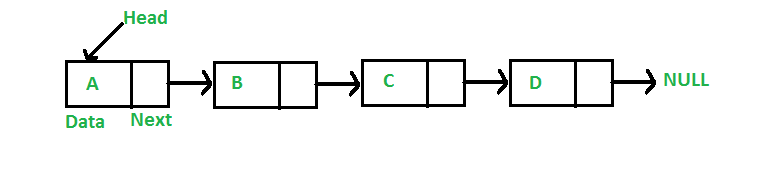
\includegraphics[width=.7\columnwidth]{fig/linked_list1.png}
    \caption{Singly Linked List}
    \label{fig:singly_linkedlist}
        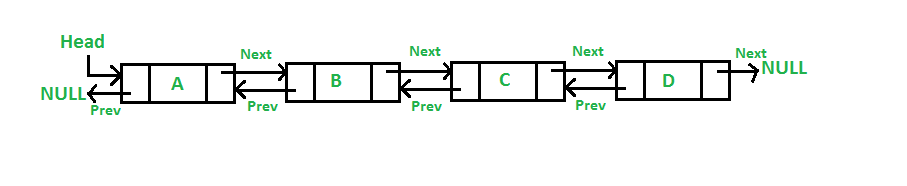
\includegraphics[width=0.9\columnwidth]{fig/DLL1.png}
    \caption{Doubly Linked List}
\end{figure}

\paragraph{Singly and Doubly Linked List} When the \texttt{node} has only one pointer, it is called \textit{singly linked list} which means we can only scan nodes in one direction; when there is two pointers, one pointer to its predecessor and another to its successor, it is called \textit{doubly linked list} which supports traversal in both forward and backward directions. 

\paragraph{Operations and Disadvantages} 
\begin{itemize}
    \item No Random access: in linked list, we need to start from some pointer and to find one item, we need to scan all items sequentially in order to find it and access it;
    \item Insertion and Deletion: only $O(1)$ to insert or delete an item if we are given the node after where to insert or the node the delete.
    \item Search and Iteration: $O(n)$ time for linked list to iterate all items. Similarly to search an item by value through iteration takes $O(n)$ time too.
    \item Extra memory space for a pointer is required with each element of the list.
\end{itemize}

\paragraph{Recursive} A linked list data structure is actually a \textit{recursive data} structure; any node can be treated as a head node thus making it a sub-linked list.  
\subsection{Stack and Queue}
\begin{figure}[!ht]
    \centering
    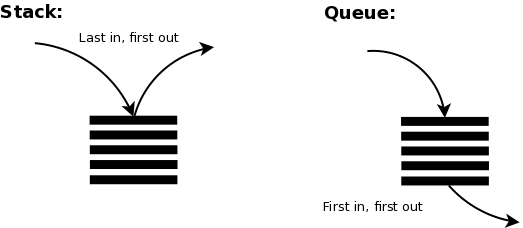
\includegraphics[width=0.7\columnwidth]{fig/stack_queue_1.png}
    \caption{Stack VS Queue}
    \label{fig:stack_queue_1}
\end{figure}
Stacks and queues are \textbf{dynamic arrays} with restrictions on deleting operation. Items adding and deleting in a stack follows the ``Last in, First out(LIFO)'' rule, and in a queue, the rule is ``First in, First out(FIFO)'', this process is shown in Fig.~\ref{fig:stack_queue_1}.  We can simply think of stack as a stack of plates, we  always put back  and fetch a plate from the top of the pile. Queue is just like a real-life queue in any line, to be first served with your delicious ice cream, you need to be there in the head of the line. 


Implementation-wise, stacks and queues are a simply dynamic array that we add item by appending at the end of array, and they only differs with the delete operation: for stack, we delete item from the end; for a queue, we delete item from the front instead. Of course, we can also implement with any other linear data structure, such as linked list. Conventionally, the add and deletion operation is called  ``push'' and ``pop'' in a stack, and ``enque'' and ``deque'' in a queue.

\paragraph{Operations} Stacks and Queues support limited access and limited insertion and deletion and the search and iteration relies on its underlying data structure. 


Stacks and queues are widely used in computer science. First, they are used to implement the three fundamental searching strategies--Depth-first, Breath-first, and Priority-first Search. Also, stack is a recursive data structure as it can be defined as:
\begin{itemize}
    \item a stack is either empty or
    \item it consists of a top and the rest which is a stack;  
    \end{itemize}

\subsection{Hash Table}
\begin{figure}[h!]
    \centering
    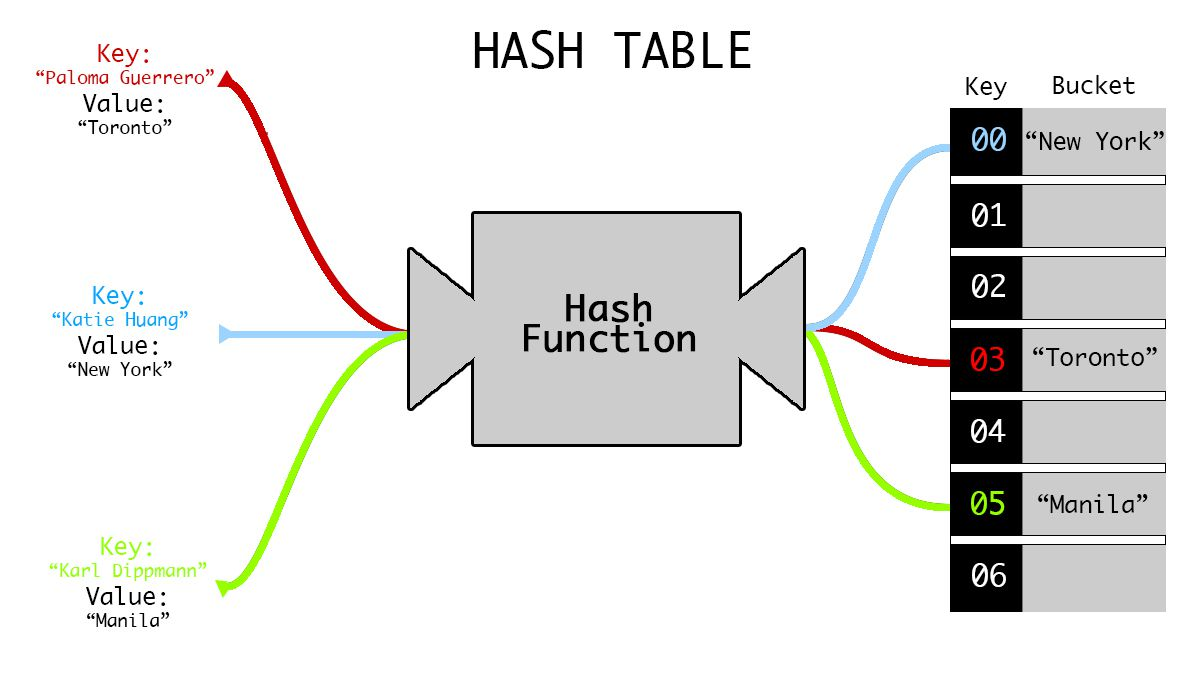
\includegraphics[width=0.6\columnwidth]{fig/hash_table_1.png}
    \caption{Example of Hashing Table, replace key as index}
    \label{fig:hash_table_1}
\end{figure}
A hash table is a data structure that (a) stores items formed as  \{key: value\} pairs, (b) and uses a \textit{hash function} $index=h(key)$ to compute an index into an array of buckets or slots, from which the mapping value will be stored and accessed; for users, ideally, the result is given a key we are expected to find its value in constant time--only by computing the hash function. An example is shown in Fig.~\ref{fig:hash_table_1}. Hashing will not allow two pairs that has the same key.

First, the key needs to be of real number; when it is not, a conversion from any type it is to a real number is necessary. Now, we assume the keys passing to our hash function are all real numbers. We define a \textit{universe} set of keys $U=\{0,1,2,...,|U-1|\}$. To frame hashing as a math problem: given a set of keys drawn from $U$ that has n \{key: value\} pairs, a hash function needs to be designed to map each pair to a key in a set in range $\{0,..,m-1\}$ so that it fits into a table with size m (denoted by $T[0...m-1]$), usually $n>m$. We denote this mapping relation as $h:U\xrightarrow{}\{0,...,m-1\}$. The simplest hashing function is $h=key$, called \textit{direct hashing}, which is only possible when the keys are drawn from $\{0,...,m-1\}$ and it is usually not the case in reality.

Continue from the hashing problem, when two keys are mapped into the same slot, which will surely happen given $n>m$, this is called \textit{collision}. In reality, a well-designed hashing mechanism
should include: (1) a hash function which minimizes the number of collisions
and (2) a efficient collision resolution if it occurs.
\subsubsection{Hashing Functions}
The essence of designing hash functions is uniformity and randomness. We further use $h(k,m)$ to represent our hash function, which points out that it takes two variables as input, the key as $k$, and $m$ is the size of the table where values are saved. One essential rule for hashing is if two keys are equal, then a hash function should produce the same key value ($h(s, m)=h(t, m)$, if $s=t$). And, we try our best to minimize the collision to make it unlikely for two distinct keys to have the same value. Therefore our expectation for average collision times for the same slot will be $\alpha= \frac{n}{m}$, which is called \textbf{loading factor} and is a critical statistics for design hashing and analyze its performance. Besides,
a good hash function satisfied the condition of simple uniform hashing: each key is equally likely to be mapped to any of the $m$ slots. But usually it is not possible to check this condition because one rarely knows the probability distribution according to which the keys are drawn. There are generally four methods: 
\begin{enumerate}
    \item \textbf{The Direct addressing method}, $h(k, m) = k$, and $m=n$. Direct addressing can be impractical when n is beyond the memory size of a computer. Also, it is just a waste of spaces when $m<<n$. 
    \item \textbf{The division method}, $h(k, m) = k \% m$, where $\%$ is the module operation in Python, it is the reminder of $k$ divided by $m$. A large prime number not too close to an exact power of 2 is often a good choice of $m$. The usage of prime number is to  minimize collisions when the data exhibits some particular patterns. For example, in the following cases, when $m=4$, and $m=7$, keys = [10, 20, 30, 40, 50]
    \begin{lstlisting}[numbers=none]
           m = 4      m  = 7
    10   10=4*2+2      10=7*1+3
    20   20=4*5+0      20=7*2+6
    30   30=4*7+2      30=7*4+2
    40   40=4*10+0     40=7*5+5
    50   50=4*12+2     50=7*7+1
    \end{lstlisting}
    Because the keys share a common factor $c=2$ with the bucket size  $m=4$, this will decrease the range of the reminder into $m/c$ of its original range.
    %proof(They key can be recomputed from the quotient $q$ from $k/m$, the reminder $r$ from $k\%m$, and $m$ as $k=q*m+r$. Further we write $r=k-q*m$. Because of the common factor, we write $k=p\times c, m=a\times c$, we can get $\frac{m}{r}=\frac{qc}{pc-qac}=\frac{a}{p-qa}=\frac{m/c}{k/c-\lfloor k/m\rfloor m/c}=m/c$; this decrease the range of the reminder into  $[0, m/c]$.) 
    As shown in the example, the remainder is just \{0, 2\} which is only half of the space of m. The real loading factor increase to $c\alpha$. Using a prime number is a easy way to avoid this since a prime number has no factors other than 1 and itself.
    
    If the size of table cannot easily to be adjusted to a prime number, we can use $h(k, m) = (k \% p) \% m$, where $p$ is our prime number which should be chosen from the range $m<p<|U|$.
    \item \textbf{The multiplication method}, $h(k, m)=\lfloor m(kA \% 1)\rfloor$. $A \in (0, 1)$ is a chosen constant and a suggestion to it is $A=(\sqrt{5}-1)/2$. $kA \% 1$ means the fractional part of $kA$  which equals to $kA-\lfloor kA \rfloor$. It is also shorten as $\{kA\}$. For example, the fractional part of $45.2$  is $.2$. In this case, the choice of $m$ is not as critical as in the division method; for convenience, it is suggested with $m=2^p$, where $p$ is some integer. 
    \item \textbf{Universal hashing method}: because any fixed hash function is vulnerable to the worst-case behavior when all $n$ keys are hashed to the same index, an effective way is to choose the hash function randomly from a set of predefined hash functions for each execution--the same hash function must be used for all accesses to the same table. However, finding the predefined hash functions requires us to define multiple prime numbers if the division method for each function is used, which is not easy. A replacement is to define $h(k, m) = ((ak+b) \% p) \% m, a, b<p$, $a,b$ are both integers.
\end{enumerate}

\subsubsection{Resolving Collision}
Collision is unavoidable given that $m<n$ and the sometimes it just purely bad luck that the data you have and the chosen hashing function produce lots of collisions, thus, we need mechanisms to resolve possible collisions. We introduce three methods: Chaining, Open Addressing, and Perfect Hashing.
\paragraph{Chaining}
\begin{figure}[ht!]
    \centering
    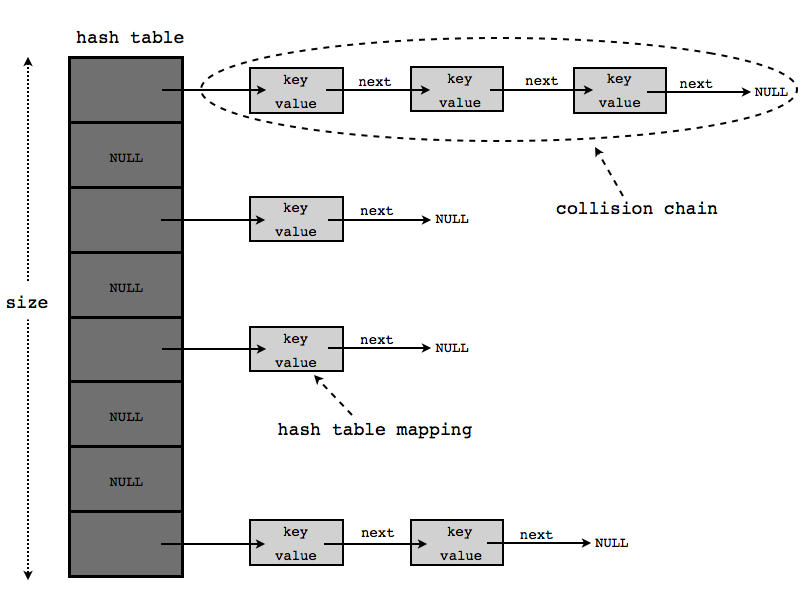
\includegraphics[width = 0.6\columnwidth]{fig/hashtable_chaining.png}
    \caption{Hashtable chaining to resolve the collision, change it to the real example}
    \label{fig:chaining}
\end{figure}
An easy way to think of is by chaining the keys that have the same hashing value using a linked list (either singly or doubly). For example, when $h(k, m)= k\%4$, and keys = [10,20,30,40,50]. For key as 10, 30, 50, they are mapped to the same slot 2. Therefore, we chain them up at index 2 using a single linked list shown in Fig.~\ref{fig:chaining}.  This method shows the following characters:
\begin{itemize}
    \item The average-case time for searching is $O(\alpha)$ under the assumption of simple uniform hashing. 
    \item The worst case running time for insertion is $O(1)$.
    \item the worst-case behavior is when all keys are mapped to the same slot. 
\end{itemize}


The advantage of chaining is the flexible size because we can always add more items by chaining behind, this is useful when the size of the input set is unknown or too large. However, the advantage comes with a price of taking extra space due to  the use of pointers.
\paragraph{Open Addressing}
In Open addressing,  all items are stored in the hash table itself; thus requiring the size of the hash table to be ($m\ge n$), making each slot either contains an item or empty and the load factor $\alpha\leq1$. This avoids the usages of pointers, saving spaces. So, here is the question, what would you do if there is collision?
\begin{itemize}
    \item Linear Probing: Assume, at first, from the hash function, we save an item at $h(k_1,m)=p_1$, when another pair $\{k_2,v_2\}$ comes, we have index $h(k_2,m)$. If the index is the same as $k_1$, we can simply check the position right after $p_1$ in a cyclic order(from $p_1$ to the end of hash table, continue from the start of the table and end at $p_1-1$): if it is empty, we save the value at $p_1+1$, otherwise, we try $p_1+2$, and so on until we find an empty spot, this is called \textit{linear probing}. However, there are other keys such as $k_3$ that is mapped to index $p_1$ at the first time too, for $k_3$, it would collide with $k_1$ at $p_1$, with $k_2$ at $p_1+1$, and the second collision is called \textit{secondary collision}. When the table is relative full, such secondary collision can degrade the searching in the hashing table to linear search. We can denote the linear probing as
\begin{equation}
    h'(k,i,m)=(h(k,m)+i)\%m, \texttt{for } i=0, 1, 2, ..., m-1.
\end{equation}
$i$ marks the number of tries. Now, try to delete item from linear probing table, we know  that $T[p_1] = k_1, T[p_1+1] = k_2, T[p_1+2] = k_3$.  say we delete $k_1$, we repeat the hash function, find and delete it from $p_1$, working well, we have $T[p_1==NULL$. Then we need to delete or search for $k_2$, we first find $p_1$ and find that it is empty already, then we thought $k_2$ is deleted, great! You see the problem here? $k_2$ is actually at $p_1+1$ but from the process we did not know. A simple resolution instead of really deleting the value, we add a flag, say \texttt{deleted}, at any position that a key is supposedly be deleted. Now, to delete $k_1$, we have $p_1$ is marked as \texttt{deleted}. This time, when we are trying to delete $k_2$, we first go to $p_1$ and see that the value is not the same as its value, we would know we should move to $p_1+1$, and check its value: it equals, nice, we put a marker here again. 

\item *Other Methods: However, even if the linear probing works, but it is far from perfection. We can try to decrease the secondary collisions using \textit{quadratic probing} or \textit{double hashing}.
\end{itemize}

In open addressing, it computes a probe sequence as of [h(k, m, 0), h(k, m, 1),...,h(k,m, m-1)] which is a permutation of [0, 1, 2, ..., m-1]. We successively probe each slot until an empty slot is found. 

\paragraph{*Perfect Hashing}
%%%%%%%%%%%%%%%%%%Graphs%%%%%%%%%%%%%%%%%%%%%%
\section{Graphs}
\label{chapter_abstract_data_structure_graphs}
\subsection{Introduction}
\begin{figure}[!ht]
    \centering
        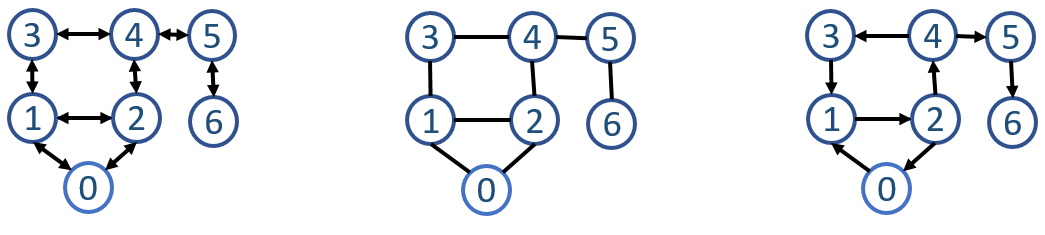
\includegraphics[width=\columnwidth]{fig/example_undirected_directed_graph.png}
    \caption{Example of graphs. Middle: undirected graph, Right: directed graph, and Left: representing undirected graph as directed, Rightmost: weighted graph.}
    \label{fig:graph_2}
\end{figure}
Graph is a natural way to represent connections and reasoning between things or events. A graph is made up of \textit{vertices} (nodes or points) which are connected by \textit{edges} (arcs or lines). A graph structure is shown in Fig.~\ref{fig:graph_2}.  We use $G$ to denote the graph, $V$ and $E$ to refer its collections of vertices and edges, respectively. Accordingly, $|V|$ and $|E|$ is used to denote the number of nodes and edges in the graph.  An edge between vertex $u$ and $v$ is denoted as a pair $(u, v)$, depending on the type of the graph, the pair can be either ordered or unordered. 

There are many fields in that heavily rely on the graph, such as the probabilistic graphical models applied in computer vision, route problems, network flow in network science, link structures of a website in social media, and so. We present graph as a data structure. However, graph is really a broad way to model problems; for example, we can model the possible solution space as a graph and apply graph search to find the possible solution to a problem.  So, do not let the physical graph data structures limit our imagination. 

The representation of graph is deferred to Chapter.~\ref{chapter_code_graph}. In the next section, we introduce the types of graphs. 

% In Fig.~\ref{fig:graph_2}, all our graphs have 7 vertices and 8 edges in the middle and right graph.  The \textit{weights of edges} refers to the information with edges. 

\subsection{Types of Graphs}
\paragraph{Undirected Graph VS Directed Graph} If one edge is directed that it points from $u$(the tail) to $v$ (the arc head), but not the other way around, this means we can reach to $v$ from $u$, but not the opposite.  An ordered pair $(u, v)$ can denote this edge, in this book, we denote it as $(u \rightarrow v)$. If all edges are directed, then we say it is a directed graph as shown on the right of Fig.~\ref{fig:graph_2}. If all edges $e \in E $ is an unordered pair $(u, v)$, that it is reachable from both way for  $u, v \in V$ then the graph is undirected graph as shown in the middle of Fig.~\ref{fig:graph_2}. 

\paragraph{Unweighted Graph VS Weighted Graph} In \textit{weighted} graphs, each edge of $G$ is assigned a numerical value, or weighted. For example, the road network can be drawn as a directed and weighted graph: two edges if it is a two-way road, and one arc if its is one-way instead; and the weight of an edge might be the length, speed limit or traffic. In \textit{unweighted} graphs, there is no cost distinction between various edges and vertices. 

\paragraph{Embedded Graph VS Topological Graph} A graph is defined without a geometric position of their own, meaning we literally can draw the same graph with vertices arranged at different positions. We call a specific drawing of a graph as an embedding, and trawn graph is called embedded graph. Occasionally, the structure of a graph is completely defined by the geometry of its embedding, such as the famous travelling salesman problem, and  grids of points are another example of topology from geometry. Many problems on an $n \times m$ grid involve walking between neighboring points, so the edges are implicitly defined from the geometry.

\paragraph{Implicit Graph VS Explicit Graph} Certain graphs are not explicitly constructed and traversed, but it can be modeled as a graph. For example, grids of points can also be looked as implicit graph, where each point is an vertex and usually a point can link to its neighbors through an implicit edge. Working with implicit graph takes more imagination and practice. Another example will be seen in the backtracking as we are going to learn in Chapter~\ref{chapter_non_linear_graph}, the vertices of the implicit graph are the states of  the search vector while edges link pair of states that can be directly generated from each other. It is totally ok that you do not get it right now, relax, come back and think about it later.  

\paragraph{Terminologies of Graphs}  In order to apply graph abstractions in real problems, it is important to get familiar with the following important terminologies of graphs: 
\begin{enumerate}
    \item \textbf{Path:} A path in a graph is a sequence of adjacent vertices. For example, there is a path $(0, 1, 2, 4)$ in both the undirected and directed graph in Fig.~\ref{fig:graph_2}.  The length of a path in an unweighted graph is the total number of edges that it passes through--i.e., it is one less than the number of vertices in the graph. A \textit{simple path} is a path with no repeated vertices. In the weighted graph, it may instead be the sum of the weights of all of its consisting edges. Obtaining the shortest path can be a common task and of real-value. 
    \item \textbf{cycles:} In directed graph a \textit{cycle} is a path that starts and ends at the same vertex, and in undirected graph. A cycle can have length one, i.e. a \textit{selfloop}. A \textit{simple cycle} is a cycle that has no repeated vertices other than the start and the end vertices being the same.   In an undirected graph a (simple) cycle is a path that starts and ends at the same vertex, has no repeated vertices other than the first and last, and
has length at least three. In this book we will exclusively talk about simple cycles and hence, as
with paths, we will often drop simple. A graph is \textit{acyclic} if it contains no cycles. Directed acyclic graphs are often abbreviated as \textbf{DAG}.
\item \textbf{Distance:} The \textit{distance} $\sigma(u, v)$ from a vertex $u$ to a vertex $v$ in a graph $G$ is the shortest path (minimum number of edges) from $u$ to $v$. It is also referred to as the \textit{shortest path length} from $u$ to $v$. 
\item \textbf{Diameter:} The \textit{diameter} of a graph is the maximum shortest path length over all pairs of vertices: $diam(G) = \max{\sigma(u, v): u, v \ in V}$.
    \item \textbf{Tree:} An acyclic and undirected graph is a \textit{forest} and if it is connected it is called a \textit{tree}. A \textit{rooted tree} is a tree with one vertex designated as the root. A tree can be directed graph too, and the edges are typically all directed toward the root or away from the root.  We  will detail more in the next section.
    \item \textbf{Subgraph:} A \textit{subgraph}  is another graph whose vertices $V_s$ and  edges $E_s$  are subsets of $G$, and all endpoints of $E_s$ must be included in $E_s$-- $V_s$ might have  additional vertices. When $V=V_s, E_s \subset E$, that the subgraph includes all vertices of graph $G$ is called  \textbf{A spanning subgraph}; when $E_s=E, V_s\subset V$, that the subgraph contains all the edges whose endpoints belong the vertex subset is called \textbf{an induced subgraph}. 
    % \item \textbf{Supergraph:} A graph formed by adding vertices, edges, or both to a given graph. If H is a subgraph of G, then G is a supergraph of H. 
    \item \textbf{Complete Graph:} A graph in which each pair of graph vertices is connected by an edge is a complete graph. A complete graph with $|V|$ vertices is denoted as $K_n = (|C|, 2) = n(n-1)/2$, pointing out that it will has $(|V|,2)$ total edges. 
    
    \begin{figure}[!ht]
    \centering
    % 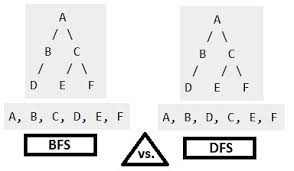
\includegraphics[width=0.6\columnwidth]{fig/dfs_bfs.png}
    % \caption{BFS VS DFS}
    % \label{fig:bfs_dfs}
    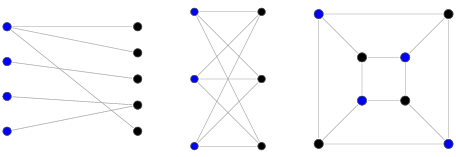
\includegraphics[width=0.7\columnwidth]{fig/BipartiteGraph_1000.png}
    \caption{Bipartite Graph}
    \label{bipartite_graph}
\end{figure}
    \item \textbf{Bipartite Graph:} A bipartite graph, a.k.a bigraph, is a graph whose vertices can be divided into two disjoint sets $V_1$ and $V_2$ such that no two vertices within the same set are connected to each other or adjacent. A bipartite graph is a graph with no odd cycles; equivalently, it is a graph that may be properly colored with two colors. See Fig.~\ref{bipartite_graph}.
    \item \textbf{Connected Graph:} A graph is connected if there is a path joining each pair of vertices, that it is always possible to travel in a connected graph between one vertex and any other. If a graph is not fully connected, but has subset $V_s$ that are connected, then the connected parts of a graph are called its \textbf{components}. 

\end{enumerate}

\subsection{Reference}
\begin{enumerate}
    \item \url{http://www.cs.cmu.edu/afs/cs/academic/class/15210-f14/www/lectures/graph-intro.pdf}
\end{enumerate}
%%%%%%%%%%%%%%%%%%%%%Tree%%%%%%%%%%%%%%%%%%%%%%%%%%%%%%%%%%%
\section{Trees}
\label{chapter_abstract_data_structure_trees}

\paragraph{Trees in Interviews} The most widely used are binary tree and binary search tree which are also the most popular tree problems you encounter in the real interviews.
A large chance you will be asked to solve a binary tree or binary search tree related problem in a real coding interview especially for new graduates which has no real industrial experience and pretty much had no chance before to put the major related knowledge into practice yet. 
\subsection{Introduction}
A tree is essentially a simple graph which is (1) connected, (2) acyclic, and (3) undirected. To connect $n$ nodes without a cycle, it requires $n-1$ edges. Adding one edge will create one cycle and removing one edge will divides a tree into two components. Trees can be represented as a graph whose representations we have learned in the last section,  such a tree is called \textit{free tree}.  A \textbf{Forest} is a set of $n>=0$ disjoint trees. 

\begin{figure}[!ht]
    \centering
    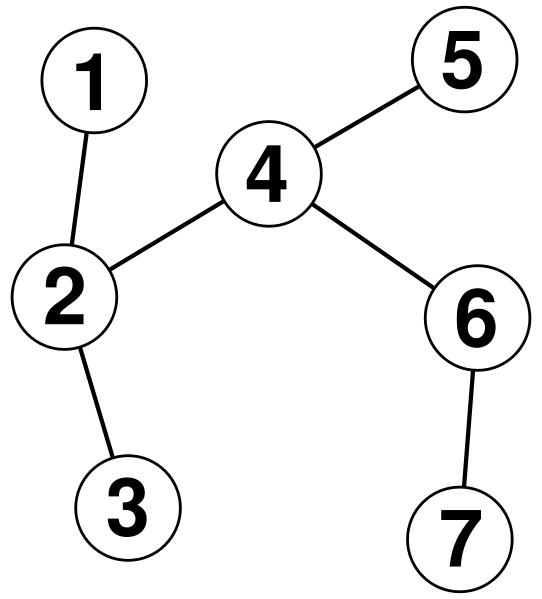
\includegraphics[width=0.4\columnwidth, height=5cm]{fig/542px-Graph_theory_tree.png}
    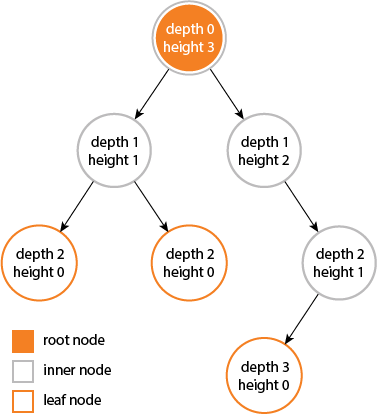
\includegraphics[width=0.55\columnwidth, height=5cm]{fig/tree_property.png}
    \caption{Example of Trees. Left: Free Tree, Right: Rooted Tree with height and depth denoted}
    \label{fig:tree_property}
\end{figure}
However, free trees are not commonly seen and applied in computer science (not in coding interviews either) and there are better ways--\textit{rooted trees}. In a  {rooted tree}, a special node is singled out which is called the \textit{root} and all the edges are oriented to point away from the root. The rooted node and one-way structure enable the rooted tree to indicate a hierarchy relation between nodes whereas not so in the free tree. A comparison between free tree and the rooted tree is shown  in Fig.~\ref{fig:tree_property}.



\subsubsection{Rooted Trees}  A rooted tree introduces a \textbf{parent-child}, \textbf{sibling relationship} between nodes to indicate the hierarchy relation.  
%In general purposed programming and the coding interviews, a rooted tree is more widely used compared with the free tree. Thus, the rooted trees are one of the well-known  non-linear data structures. They organize data hierarchically other than in the linear way. 

\paragraph{Three Types of Nodes} Just like a real tree, we have the root, branches, and finally the leaves. The first node of the tree is called the \textbf{root node}, which will likely to be connected to its several underlying children node(s), making the root node the parent node of its children. Besides the root node, there are another two kinds of nodes: \textit{inner nodes} and \textit{leaf nodes}. A leaf node can be found at the last level of the tree which has no further children.  An inner node is any node in the tree that has both parent node and children, which is also any node that can not be characterized as either leaf or root node. A node can be both root and leaf node at the same time, if it is the only node that composed of the tree. 

\paragraph{Terminologies of Nodes} We define the following terminologies to characterize nodes in a tree.
\begin{itemize}
    \item \textbf{Depth:} The \textit{depth} (or level) of a node is the number of edges from the node to the tree's root node. The depth of the root node is $0$. % and the depth of all nodes can be obtained from up-down level-by-level traversal.
    \item \textbf{Height:} The \textit{height} of a node is the number of edges on the \textit{longest path} from the node to a leaf. A leaf node will have a height of $0$.
    \item \textbf{Descendant:} The \textit{descendant} of a node is any node that is reachable by repeated proceeding from parent to child starting from this node. They are also known as \textit{subchild}.
    \item \textbf{Ancestor:} The \textit{ancestor} of a node is any node that is reachable by repeated proceeding from child to parent starting from this node.
    \item \textbf{Degree:} The \textbf{degree} of a node is the number of its children. A leaf is necessarily degreed zero. 
\end{itemize}

\paragraph{Terminologies of Trees} Following the characteristics of nodes, we further define some terminologies to describe a tree. 
\begin{itemize}
    \item \textbf{Height:} The \textit{height}(or \textit{depth}) of a tree would be the height of its root node, or equivalently, the depth of its deepest node. 
    \item \textbf{Diameter:} The \textit{diameter} (or \textit{width}) of a tree is the number of nodes (or edges) on the longest path between any two leaf nodes. 
    \item \textbf{Path:} A \textit{path} is defined as a sequence of nodes and edges connecting a node with a descendant.  We can classify them into three types: 
\begin{enumerate}
    \item Root->Leaf Path: the starting and ending node of the path is the root and leaf node respectively;
    \item Root->Any Path: the starting and ending node of the path is the root and any node (inner, leaf node) respectively;
    \item Any->Any Path: the starting and ending node of the path is both any node (Root, inner, leaf node) respectively. 
\end{enumerate}
\end{itemize}

\paragraph{Representation of Trees}   Like linked list, which chains nodes together via pointers--once the first node is given, we can get hold of information of all nodes, a rooted tree can be represented with nodes consisting of pointers and values too. Because in a tree, a node would have multiple children, indicating a node can have multiple pointers.  Such representation makes a rooted tree  a \textit{recursive} data structure: each node can be viewed as a root node, making this node and all the nodes that reachable from this node a subtree of its parent. This recursive structure is the main reason we separate it from graph field, and make it one of its own data structure. The advantages are summarized as:
\begin{itemize}
    \item A tree is an easier data structure that can be recursively represented as a root node connected with its children. 
    \item Trees can be always used to organize data and can come with efficient information retrieval. Because of the recursive tree structure, divide and conquer can be easily applied on trees (a problem can be most likely divided into subproblems related to its subtrees).  For example, Segment Tree, Binary Search Tree, Binary heap, and for the pattern matching, we have the tries and suffix trees. 
\end{itemize}

The recursive representation is also called \textit{explicit} representation. The counterpart--\textit{implicit} representation will not use pointer but with array, wherein the connections are implied by the positions of the nodes. We will see how it works in the next section. 

\paragraph{Applications of Trees}
Trees have various applications due to its convenient recursive data structures which related the trees and one fundamental algorithm design methology-Divide and Conquer. We summarize the following important applications of trees:

\begin{enumerate}
    \item Unlike arrays and linked list, tree is hierarchical: (1) we can store information that naturally forms hierarchically, e.g., the file systems on a computer, the employee relation in at a company. (2) If we organize keys of the tree with ordering, e.g. Binary Search Tree, Segment Tree, Trie used to implement prefix lookup for strings. 
    \item Trees are relevant to the study of analysis of algorithms not only because they implicitly model the behavior of recursive programs but also because they are involved explicitly in many basic algorithms that are widely used. 
    \item Algorithms applied on graph can be analyzed with the concept of tree, such as the BFS and DFS can be represented as a tree data structure, and a spanning tree that include all of the vertices in the graph. These trees are the basis of other kind of computational problems in the field of graph. 
\end{enumerate}

\begin{importantnote}
Tree is a recursive structure, it can almost used to visualize any recursive based algorithm design or even computing the complexity in which case it is specifically called \textit{recursion tree}.
\end{importantnote}

\subsection{N-ary Tres and Binary Tree}
\begin{figure}[!ht]
    \centering
    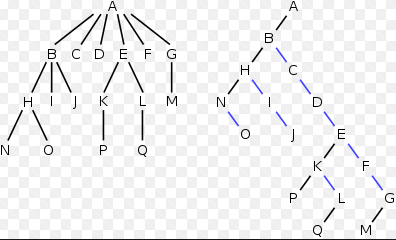
\includegraphics[width = 0.6\columnwidth]{fig/n-ary_binary_tree.png}
    \caption{A 6-ary Tree Vs a binary tree.}
    \label{fig:nary_vs_binary}
\end{figure}
For a rooted tree, if each node has no more than $N$ children, it is called \textit{N-ary} Tree. When $N=2$, it is  further distinguished as a \textit{binary tree}, where its possible two children are typically called \textit{left child} and \textit{right child}. Fig.~\ref{fig:nary_vs_binary} shows a comparison of a 6-ary tree and a binary tree. Binary tree is more common than N-ary tree because it is simplier and more concise, thus making it more popular for coding interviews.  
% \subsubsection{N-ary Tree}

% \subsubsection{Binary Tree}
% A binary tree is one of the most typical tree structure. A binary tree is made of nodes which has at most two branches--the ``left child" and the ``right child"--and a data element. The ``root" node is the topmost node in the tree. The left and right child recursively point to smaller ``subtrees" on either side. 
\begin{figure}[!ht]
    \centering
    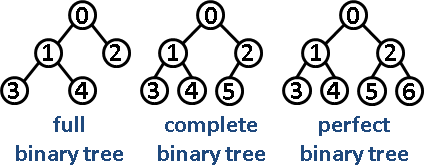
\includegraphics[width = 0.8\columnwidth]{fig/full_complete_perfect_binary_tree.png}
    \caption{Example of different types of binary trees}
    \label{fig:binary_tree_type}
\end{figure}
\paragraph{Types of Binary Tree}
There are four common types of Binary Tree:
\begin{enumerate}
    \item \textbf{Full Binary Tree:} A binary tree is full if every node has either 0 or 2 children. We can also say that a \textbf{full} binary tree is a binary tree in which all nodes except leaves have two children.  In full binary tree, the number of leaves ($|L|$)  and the number of all other non-leaf nodes ($|NL|$) has relation: $|L| = |NL| + 1$. The total number of nodes compared with the height $h$ will be:
    \begin{align}
        n &=2^0+2^1+2^2+...+2^h\\
        &= 2^{h+1}-1
    \end{align}
    \item \textbf{Complete Binary Tree:} A Binary Tree is \textbf{complete} if all levels are completely filled except possibly the last level and the last level has all keys as left as possible.
    
    \item \textbf{Perfect Binary Tree:} A Binary tree is \textbf{perfect} in which all internal nodes have two children and all leaves are at the same level. This also means a perfect binary tree is both a full and complete binary tree.
    
    \item \textbf{Balanced Binary Tree:} A binary tree is balanced if the height of the tree is $O(\log n)$ where $n$ is the number of nodes. For Example, \textit{AVL tree} maintains $O(\log n)$ height by making sure that the difference between heights of left and right subtrees is at most 1.
    
    \item Degenerate (or pathological) tree:  A Tree where every internal node has one child. Such trees are performance-wise same as linked list.
\end{enumerate}
And each we show one example in Fig.~\ref{fig:binary_tree_type}.

Complete tree and a perfect tree can be represented with an array, and we assign index 0 for root node, and given a node with index $i$, the children will be $2*i+1$ and $2*i+2$, this is called \textit{implicit} representation, wherein its counterpart recursive representation is called \textit{explicit} representation. 






% \section{Geometric Data Structures}
% A single data point such as a real number 8 is called a \textit{scalar}, and an array of items can be a \textit{vector}, which is one dimensional, a two dimensional data such as an image, needed to be represented with a \textit{matrix}. To find where each data point is in the dimensional data structures, we build up \textit{coordinates} with dimensions and use \textit{point} to mark the position in the geometry field.

\end{document}